\section{Обзор}

В данном разделе определены основные необходимые понятия из
теории формальных языков, рассмотрены способы сведения анализа псевдонимов и Points-to анализа, учитывающего поля, к задаче КС-достижимости, приведены решающие её алгоритмы, основанные на операциях линейной алгебры. Также приведены различные реализации, решающие задачу КС-достижимости.

\subsection{Терминология}
\textbf{Контекстно-свободная грамматика} --- $G = \langle \Sigma, N, P, S\rangle$, где:
\begin{itemize}
    \item $\Sigma$ --- множество терминальных символов;
    \item $N$ --- множество нетерминальных символов;
    \item $P$ --- множество продукций, каждая продукция имеет вид $A \to \alpha$, где $A \in N, \alpha \in (\Sigma \cup N)^* \cup {\varepsilon}$;
    \item $S \in N$ --- стартовый нетерминал.
\end{itemize}

Последовательность терминалов и нетерминалов $\gamma \alpha \delta$ \textbf{непосредственно выводится из} $\gamma \beta \delta$ \textit{при помощи правила} $\alpha \rightarrow \beta$ ($\gamma \alpha \delta \Rightarrow \gamma \beta \delta$), если:
\begin{itemize}
    \item $\alpha \rightarrow \beta \in P$;
    \item $\gamma, \delta \in \{\Sigma \cup N\}^* \cup {\varepsilon}$.
  \end{itemize}

\textbf{Отношение выводимости} является рефлексивно-транзитивным замыканием отношения непосредственной выводимости. $\alpha \derives \beta$ означает $\exists \gamma_0, \dots \gamma_k: \ \alpha \derives[] \gamma_0 \derives[] \gamma_1 \derives[] \dots \derives[] \gamma_{k-1} \derives[] \gamma_{k} \derives[] \beta$.

\textbf{Язык, задаваемый грамматикой} --- множество строк, из стартового нетерминала грамматики $\mathcal{L} (G) = \{ \omega \in \Sigma^* \mid S \derives \omega \}$.

Контекстно-свободная грамматика находится в \textbf{ослабленной нормальной форме Хомского (ОНФХ)}, если все продукции имеют вид:
\begin{itemize}
    \item либо $A \to BC$, где $A,B,C \in N$;
    \item либо $A \to a$, где $A \in N, a \in \Sigma$;
    \item либо $A \to \varepsilon$, где $A \in N$.
\end{itemize}

ОНФХ отличается от нормальной формы Хомского тем, что в ней допускаются продукции вида $A \to \varepsilon$ для любого нетерминала, а не только для стартового.

% Граф
\textbf{Ориентированный граф с метками на ребрах} $\mathcal{G} = \langle V, E, L \rangle$ есть тройка объектов, где $V$ --- конечное непустое множество вершин, $E~\subseteq~V~\times~L~\times~V$ --- конечное множество рёбер, $L$ --- конечное множество меток графа. Здесь и далее считается, что вершины графа индексируются целыми числами, то есть $V = \{0~,...,~|V| - 1\}$.

\textbf{Путь $\pi$} в графе $\mathcal{G} = \langle V, E, L \rangle$ --- это последовательность рёбер $e_0,e_1,e_{n-1}$, где ${e_i = (v_i, l_i, u_i) \in E}$, для любых ${e_i,e_{i+1}:u_i=v_{i+1}}$. Путь между вершинами $v$ и $u$ будем обозначать как $v \pi u$. Путь ${\pi=(v_0,l_0,v_1),...,(v_{n-1}, l_{n-1},v_n)}$, формирует слово $\omega (\pi) = l_0 ... l_{n-1}$.


% Рекурсивный автомат
\textbf{Рекурсивный автомат}~\cite{rsm} над конечным алфавитом $\Sigma$ есть ${R=\langle M,m,\{C_i\}_{i \in M}\rangle}$, где:

\begin{itemize}
    \item $M$ --- конечное множество меток;
    \item $m \in M$ --- начальная метка;
    \item $ \{C_i\}_{i \in M} $ --- множество \textit{конечных автоматов},
          где ${C_i=\langle\Sigma\cup M,Q_i,q_i^0,F_i,\delta_i\rangle}$:
    \begin{itemize}
        \item $\Sigma \cup M$ --- множество символов, $\Sigma \cap M = \emptyset$;
        \item $Q_i$ --- конечное множество состояний,
              где $Q_i \cap Q_j = \emptyset, \forall i \neq j$;
        \item $q_i^0$ --- начальное состояние $C_i$;
        \item $F_i$ --- множество финальных состояний $C_i$, где $F_i \subseteq Q_i$;
        \item $\delta_i$ --- функция переходов $C_i$,
              где $\delta_i: Q_i \times (\Sigma \cup M)
              \to Q_i$.
    \end{itemize}
\end{itemize}

Для ориентированного графа $\mathcal{G}$ и КС языка $\mathcal{L}$ задача \textbf{контекстно-свободной достижимости} заключается в поиске всех таких пар вершин $(v,u)$, что между ними существует путь $v \pi u$ такой, что $\omega (\pi) \in \mathcal{L}$. Результат запроса обозначается как ${R = \{ (v,u)~|~\exists v \pi u : \omega (\pi) \in \mathcal{L} \}}$.


\subsection{Анализ псевдонимов} 

Два указателя являются псевдонимами, если они указывают на одну и ту же область памяти. Задача поиска псевдонимов, нечувствительная к потоку данных, может быть выражена как задача контекстно-свободной достижимости на графе выражений программы~\cite{demand_driven_alias_analysis}. В этом графе вершинам соответствуют переменная-указатель $x$, разыменование указателя $*x$ и взятие адреса указателя $\&x$. Оператор присваивания с этими выражениями порождает рёбра по следующим правилам:

\begin{table}[H]
    \centering
    \begin{tabular}{ll}
        Выражение & Ребро в графе \\
        x = y & $x \xleftarrow{a} y$ \\
        *x = y & $*x \xleftarrow{a} y$ \\
        x = *y & $x \xleftarrow{a} *y$ \\
        x = \&y & $x \xleftarrow{a} \&y$ \\
    \end{tabular}
\end{table}

Каждая операция выделения памяти ($x=malloc(...)$) обрабатывается аналогично взятию адреса, то есть в граф добавляется ребро от выделенного участка памяти к ячейке памяти, в которую записывается указатель $x \xleftarrow{a} \&O$, где $\&O$ --- адрес выделенного участка памяти. Также для каждого указателя $x$ добавляются рёбра разыменования с меткой $d$: $x \xrightarrow{d} *x$ и $\&x \xrightarrow{d} x$.

Если достроить полученный граф обратными рёбрами: для каждого ребра $x \xrightarrow{a} y$ добавляется $x \xleftarrow{\overline{a}} y$, а для ребра $x \xrightarrow{d} y$ добавляется $x \xleftarrow{\overline{d}} y$, то такое представление программы позволяет сформулировать задачу анализа псевдонимов как задачу поиска путей с контекстно-свободными ограничениями, задаваемую грамматикой с алфавитом $\Sigma=\{a, \overline{a}, d, \overline{d}\}$, нетерминалами $N=\{\mathit{MA}, \mathit{VA}\}$, стартовым нетерминалом $\mathit{MA}$ и следующими продукциями (продукция для нетерминала $\mathit{VA}$ для краткости записана в формате, отличном от описанного выше, но может быть сведена к нему):
\begin{table}[h!]
    \centering
    \begin{tabular}{ll}
        Memory alias & $\mathit{MA} \to \overline{d}\ \mathit{VA} \ d$ \\
        Value alias & $\mathit{VA} \to (\mathit{MA}?\ \overline{a})^*\ \mathit{MA}?\ (a\ \mathit{MA}?)^*$ \\
    \end{tabular} 
\end{table}

На рис.~\ref{fig:andersen_pag} представлены пример программы и построенный по ней граф выражений. Также этот граф дополнен рёбрами, которые показывают контекстно-свободную достижимость, задаваемую грамматикой. Если в графе между вершинами $v_1$ и $v_2$ существует ребро $\mathit{MA}$, то выражения в коде, соответствующие этим вершинам, являются псевдонимами.

\begin{figure}[]
    \begin{subfigure}{.3\textwidth}
        Программа \\ \\
        $v1 = \&v2;$ \\
        $v3 = \&v1;$ \\
        $v4 = malloc(...);$ \\
        $*v2 = v4;$ \\
        $v5 = *v3;$ \\
        $v6 = *v5;$
    \end{subfigure}
    \begin{subfigure}{.65\textwidth}
        \begin{tikzpicture}[node distance=2cm] 
            \node[] (1) {$\&O$};
            \node[] (2) [right of=1] {$v4$}; 
            \node[] (3) [right of=2] {$*v2$};
            \node[] (4) [below of=3] {$v2$};
            \node[] (5) [below of=4] {$\&v2$};
            \node[] (6) [right of=5] {$v1$};
            \node[] (7) [below of=6] {$\&v1$};
            \node[] (8) [right of=7] {$v3$};
            \node[] (9) [above of=8] {$*v3$};
            \node[] (10) [right of=9] {$v5$};
            \node[] (11) [above of=10] {$*v5$};
            \node[] (12) [left of=11] {$v6$};
            \node[] (13) [above of=12] {$*v6$};
            \draw[->] (1) -- node[midway, above, sloped] {a} (2); 
            \draw[->] (2) -- node[midway, above, sloped] {a} (3); 
            \draw[dashed,->] (4) -- node[midway, left] {d} (3); 
            \draw[dashed,->] (5) -- node[midway, left] {d} (4); 
            \draw[->] (5) -- node[midway, above] {a} (6); 
            \draw[dashed,->] (7) -- node[midway, left] {d} (6); 
            \draw[->] (7) -- node[midway, above] {a} (8); 
            \draw[dashed,->] (8) -- node[midway, right] {d} (9); 
            \draw[->] (9) -- node[midway, above] {a} (10); 
            \draw[dashed,->] (10) -- node[midway, right] {d} (11); 
            \draw[->] (11) -- node[midway, above] {a} (12); 
            \draw[dashed,->] (12) -- node[midway, left] {d} (13); 
            
            \draw[dotted,<->] (1) to [out=45, in=135, looseness=1] node[midway, above] {VA} (2); 
            \draw[dotted,<->] (2) to [out=45, in=135, looseness=1] node[midway, above] {VA} (3); 
            \draw[dotted,<->] (1) to [out=-45, in=-135, looseness=1] node[midway, below] {VA} (3);
            \draw[dotted,<->,red] (3) to [out=45, in=135, looseness=1] node[midway, above,red] {MA} (13); 
            \draw[dotted,<->] (4) to [out=45, in=135, looseness=1] node[midway, above] {VA} (12); 
            \draw[dotted,<->,red] (4) to [out=-30, in=-150, looseness=0.3] node[midway, above,red] {MA} (11); 
            \draw[dotted,<->] (5) to [out=30, in=150, looseness=0.6] node[midway, above] {VA} (10); 
            \draw[dotted,<->] (5) to [out=-30, in=-150, looseness=0.5] node[midway, below] {VA} (6); 
            \draw[dotted,<->,red] (6) to [out=30, in=150, looseness=0.7] node[midway, below,red] {MA} (9); 
            \draw[dotted,<->] (7) to [out=45, in=135, looseness=1] node[midway, above] {VA} (8); 
            \draw[dotted,<->] (9) to [out=-30, in=-150, looseness=0.5] node[midway, below] {VA} (10);
            \draw[dotted,<->] (12) to [out=30, in=150, looseness=0.5] node[midway, above] {VA} (11); 
        \end{tikzpicture} 
    \end{subfigure}
    \caption{Анализ псевдонимов. Программа и её граф выражений}
    \label{fig:andersen_pag}
\end{figure}


Кроме задачи поиска всех пар псевдонимов можно выделить такие задачи, как проверка того, что два выражения являются псевдонимами, и поиск всех псевдонимов для выбранных выражений. Их можно переформулировать как задачу поиска путей с контекстно-свободными ограничениями с заданным множеством исходных вершин над тем же графом. Это позволит ускорить анализ, отказавшись от обработки неинтересующих вершин.

\subsection{Points-to анализ, учитывающий поля}
Ещё один вид анализа, который может быть сформулирован как задача поиска путей с контекстно-свободными ограничениями --- Points-to анализ, учитывающий поля, применяемый для анализа Java-программ. Он заключается в определении, на какие объекты кучи могли указывать переменные в процессе работы программы.

По исходной программе строится граф, вершины которого соответствуют объектам на куче и переменным программы, а рёбра добавляются на основании присваиваний по следующим правилам:

\begin{table}[H]
    \centering
    \begin{tabular}{ll}
        Выражение & Ребро в графе \\
        x = new Obj(); & $x \xrightarrow{alloc} h$ \\
        x = y; & $x \xrightarrow{assign} y$ \\
        x = y.f; & $x \xrightarrow{load_f} y$ \\
        x.f = y; & $x \xrightarrow{store_f} y$ \\
    \end{tabular}
\end{table}

Если достроить полученный граф обратными рёбрами: для каждого ребра $x \xrightarrow{label} y$ добавляется $x \xleftarrow{\overline{label}} y$, то такое представление программы позволяет сформулировать задачу анализа указателей как задачу поиска путей с контекстно-свободными ограничениями, задаваемую контекстно-свободной грамматикой:

\begin{table}[h]
    \centering
    \begin{tabular}{ll}
        $PointsTo\ \to\ (assign\ |\ load_f\ Alias\ store_f)^*$ $alloc$ & \\
        $Alias$ $\to$ $PointsTo$ \ $FlowsTo$ & $\forall$ f $\in$ $Fields$ \\
        $FlowsTo\ \to\ \overline{alloc}\ (\overline{assign}\ |\ \overline{store_f}\ Alias\ \overline{load_f})^*$ & \\
    \end{tabular}
\end{table}

На самом деле, это не КС-грамматика, а шаблон грамматики. Каждая программа обладает уникальным набором полей, поэтому грамматика, с помощью которой будет производиться анализ, будет получена из данного шаблона и графа, построенного по конкретной программе. Так, на рис.~\ref{fig:java_pag} представлен пример программы с тремя различными полями, построенный по ней граф выражений, дополненный рёбрами, которые показывают контекстно-свободную достижимость, задаваемую грамматикой.

\begin{figure}
    \begin{subfigure}{.3\textwidth}
        Программа \\ \\
        $v1 = new\ Obj();\ //\ h1$ \\
        $v2 = new\ Obj();\ //\ h2$ \\
        $v4 = new\ Obj();\ //\ h3$ \\
        $v6 = new\ Obj();\ //\ h4$ \\
        $v5 = v4;$ \\
        $v5 = v6;$ \\
        $v1.h = v1;$ \\
        $v2.g = v1;$ \\
        $v4.f = v2;$ \\
        $v7 = v5.f;$ \\
        $v9 = v6.f;$ \\
        $v3 = v2.g;$ \\
        $v8 = v7.g;$ \\
        $v10 = v9.g;$ \\
        $v10 = v10.h;$ \\
    \end{subfigure}
    \begin{subfigure}{.65\textwidth}
        \scalebox{0.8}{
        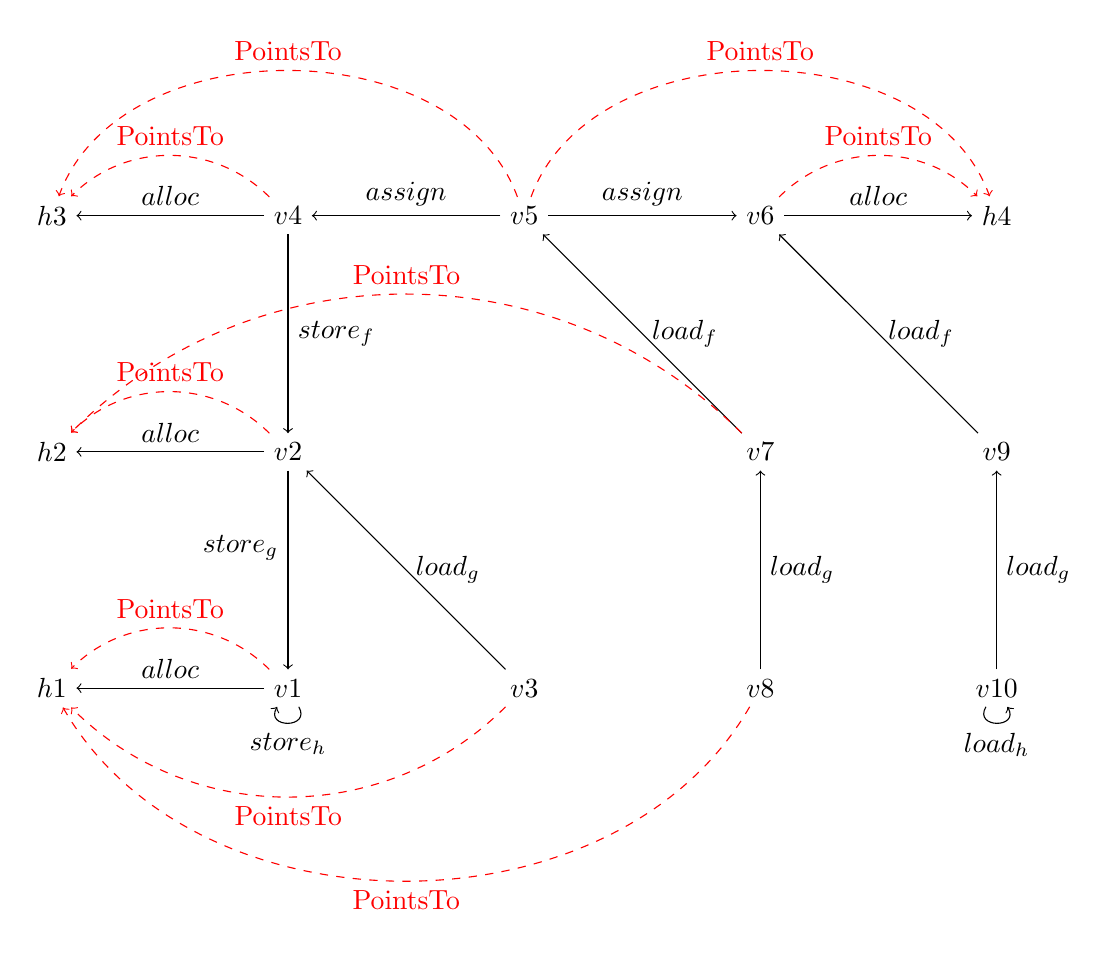
\begin{tikzpicture}[node distance=3cm] 
            \node[] (1) {$v5$};
            \node[] (2) [right of=1] {$v6$}; 
            \node[] (3) [left of=1] {$v4$};
            \node[] (4) [left of=3] {$h3$};
            \node[] (5) [right of=2] {$h4$};
            \node[] (6) [below of=3] {$v2$};
            \node[] (7) [left of=6] {$h2$};
            \node[] (8) [below of=2] {$v7$};
            \node[] (9) [below of=5] {$v9$};
            \node[] (10) [below of=6] {$v1$};
            \node[] (11) [left of=10] {$h1$};
            \node[] (12) [right of=10] {$v3$};
            \node[] (13) [below of=8] {$v8$};
            \node[] (14) [below of=9] {$v10$};
            \draw[->] (2) -- node[midway, above, sloped] {$alloc$} (5); 
            \draw[->] (3) -- node[midway, above, sloped] {$alloc$} (4); 
            \draw[->] (6) -- node[midway, above, sloped] {$alloc$} (7); 
            \draw[->] (10) -- node[midway, above, sloped] {$alloc$} (11); 
            \draw[->] (1) -- node[midway, above, sloped] {$assign$} (2); 
            \draw[->] (1) -- node[midway, above, sloped] {$assign$} (3);
            \draw[->] (14) to [out=-120, in=-60, looseness=3] node[midway, below] {$load_h$} (14); 
            \draw[->] (14) -- node[midway, right] {$load_g$} (9);
            \draw[->] (13) -- node[midway, right] {$load_g$} (8);
            \draw[->] (12) -- node[midway, right] {$load_g$} (6);
            \draw[->] (8) -- node[midway, right] {$load_f$} (1);
            \draw[->] (9) -- node[midway, right] {$load_f$} (2);
            \draw[->] (3) -- node[midway, right] {$store_f$} (6);
            \draw[->] (6) -- node[midway, above left] {$store_g$} (10);
            \draw[->] (10) to [out=-60, in=-120, looseness=3] node[midway, below] {$store_h$} (10); 
            
            \draw[dashed,->,red] (3) to [out=135, in=45, looseness=1] node[midway, above] {PointsTo} (4);
            \draw[dashed,->,red] (1) to [out=110, in=70, looseness=1] node[midway, above] {PointsTo} (4);
            \draw[dashed,->,red] (2) to [out=45, in=135, looseness=1] node[midway, above] {PointsTo} (5);
            \draw[dashed,->,red] (1) to [out=70, in=110, looseness=1] node[midway, above] {PointsTo} (5);
            \draw[dashed,->,red] (6) to [out=135, in=45, looseness=1] node[midway, above] {PointsTo} (7);
            \draw[dashed,->,red] (8) to [out=135, in=45, looseness=1] node[midway, above] {PointsTo} (7);
            \draw[dashed,->,red] (10) to [out=135, in=45, looseness=1] node[midway, above] {PointsTo} (11);
            \draw[dashed,->,red] (12) to [out=-135, in=-45, looseness=1] node[midway, below] {PointsTo} (11);
            \draw[dashed,->,red] (13) to [out=-120, in=-60, looseness=1] node[midway, below] {PointsTo} (11);
        \end{tikzpicture} 
    }
    \end{subfigure}
    \caption{Points-to анализ, учитывающий поля. Программа и её граф выражений}
    \label{fig:java_pag}
\end{figure}


\subsection{Алгоритмы КС-достижимости, основанные на операциях линейной алгебры}

Далее будут рассмотрены алгоритмы, решающие задачу контекстно-свободной достижимости, основанные на операциях линейной алгебры: матричном умножении и произведении Кронекера.

\subsubsection{Матричный алгоритм}

\begin{algorithm}
\small
\caption{Матричный алгоритм Рустама Азимова}
\label{alg:ap_matrix}
\begin{algorithmic}[1]
\Function{MatrixCFPQ}{$\mathcal{G}=(V,E,l)$, $G=(\Sigma, N, P, S)$}
    \State{$n \gets |V|$}
    \State{$M \gets \{M^A \mid  A \in N, M^A[i,j] \gets \textit{false} \text{, for all $i,j$}\} $}
    \ForAll{$v \in V$} \Comment{Инициализация матриц}
        \ForAll{$A \to \varepsilon$}
            \State{$M^A[v,v] \gets true$}
        \EndFor
    \EndFor
    \ForAll{$(v, u) \in E$} 
        \State{$label \gets l((v, u))$}
        \ForAll{$A \rightarrow label \in P$}
            \State{$M^A[u,v] \gets true$}
        \EndFor
    \EndFor    
    \While{$\exists A: M^A$ is changing}
    \Comment{Вычисление замыкания}
        \ForAll{$A \rightarrow BC \in P$}
            \State{$M^A \gets M^A + M^B \cdot M^C$}
        \EndFor
    \EndWhile
\State \Return $M^S$
\EndFunction

\end{algorithmic}
\end{algorithm}


В статье~\cite{rustam_algorithm} был преложен алгоритм, основанный на умножении матриц. На вход алгоритму подаётся граф $\mathcal{G}=\langle V,E,l \rangle$ и контекстно-свободная грамматика $G=\langle \Sigma, N, P, S\rangle$ в ослабленной нормальной форме Хомского.

Для каждого нетерминала $A \in N$ создаётся матрица смежности $M^A$. Если $M^A[i,j] = true$, то в графе между вершинами с номерами $i$ и $j$ существует путь, конкатенация меток на рёбрах которого образует слово, выводимое из нетерминала $A$ в заданной грамматике. Инициализация матриц происходит с помощью $\varepsilon$-правил: для правил вида $A \to \varepsilon$ для всех вершин добавляется петля $M^A[i,i] = true$, и простых правил грамматики (правил вида $A \to a$): если в графе между вершинами $i$ и $j$ есть ребро с меткой $a$, то $M^A[i,j] = true$.

Затем происходит поиск транзитивного замыкания (строки 15--19 алгоритма~\ref{alg:ap_matrix}), для правил вида $A \to BC$ матрица смежности нетерминала $A$ обновляется следующим образом: $M^A = M^A + M^B \cdot M^C$. Алгоритм использует булевы матрицы, поэтому в качестве сложения её элементов используется дизъюнкция, а в качестве умножения --- конъюнкция.

Результатом работы алгоритма является матрица смежности для стартового нетерминала --- $M^S$. Эта матрица будет содержать в себе информацию о всех парах вершин, соединённых путями, метки на рёбрах которых образуют слово из языка грамматики.


\subsubsection{Тензорный алгоритм}

Ещё один алгоритм КС-достижимости, основанный на операциях линейной алгебры --- алгоритм, основанный на произведении Кронекера~\cite{tensor_algorithm}. Алгоритм (листинг~\ref{alg:ap_tensor}) принимает граф $\mathcal{G}$ и рекурсивный автомат $R$. Его идея заключается в использовании модификации алгоритма пересечения конечных автоматов~\cite{automata_theory} для пересечения рекурсивного автомата и графа. Для этого граф $\mathcal{G}$ рассматривается как автомат: вершины считаются состояниями, а дуги --- переходами.

Входной граф и рекурсивный автомат представляются в виде композиции булевых матриц смежности для всех меток на рёбрах графа и переходах автомата. Пересечение выполняется с использованием произведения Кронекера, а множество рекурсивных вызовов учитывается с помощью транзитивного замыкания.

После инициализации матриц смежности проверяется наличие состояний в автомате $R$, которые одновременно являются стартовыми и конечными, и при наличии таковых для каждой вершины графа добавляется петля с соответствующей меткой.

Основной цикл алгоритма выполняется, пока набор матриц смежности для графа меняется. Первым шагом цикла происходит вычисление произведения Кронекера, тем самым создаётся матрица смежности нового автомата. Далее результат транзитивно замыкается для получения информации о достижимости состояний в полученном автомате. И последним шагом происходит обновление матрицы смежности графа.

\begin{algorithm}[]
    \small
    \begin{algorithmic}[1]
    \caption{Алгоритм, основанный на произведении Кронекера}
    \label{alg:ap_tensor}
    \Function{contextFreePathQuerying}{$\mathcal{G}$, $R$}
        % Input data preparation
        \State{$M_1 \gets$ набор матриц смежности для $R$} \Comment{Инициализация матриц}
        \State{$M_2 \gets$ набор матриц смежности для $\mathcal{G}$}
        \State{$n \gets$ dim$(M_1) \times $dim$(M_2)$}
        
        % Eps-transition handling for graph
        \For{$s \in 0..dim(\mathcal{M}_1)-1$}
            \For{$S \in \textit{getNonterminals}(R,s,s)$}
                \For{$i \in 0..dim(\mathcal{M}_2)-1$}
                    \State{$M_2^S[i,i] \gets \{1\}$}
                \EndFor
            \EndFor
        \EndFor
        \While{$M_2$ is changing} \Comment{Тело алгоритма}
            \State{$M_3 \gets M_1 \otimes M_2$} \Comment{Произведение Кронекера}
            \State{$C_3 \gets \textit{transitiveClosure}(M_3)$}
            \For{$i \in 0..n-1, j \in 0..n-1$}
                \If{$C_3[i,j]$}
                    \State{$s, f \gets \textit{getStates}(C_3,i,j)$}
                    \State{$x, y \gets \textit{getCoordinates}(C_3,i,j)$}
                    \For{$Nonterm \in \textit{getNonterminals}(R,s,f)$}
                        \State{$M_2^{Nonterm}[x,y] \gets \{1\}$}
                    \EndFor
                \EndIf
            \EndFor
        \EndWhile
    \State \Return $M_2$
    \EndFunction
    
    \Function{getStates}{$M_1, i, j$} \Comment{Получение номеров состояний автомата по номерам ячеек в матрице}
        \State{$r \gets dim(M_1)$}
        \State \Return{$\left\lfloor{i / r}\right\rfloor, \left\lfloor{j / r}\right\rfloor$}
    \EndFunction
    \Function{getCoordinates}{$M_2, i, j$} \Comment{Получение номеров вершин графа по индексам ячеек в матрице}
        \State{$n \gets dim(M_2)$}
        \State \Return{$i \bmod n, j \bmod n$}
    \EndFunction
    \end{algorithmic}
\end{algorithm}

\subsubsection{Инкрементальная версия тензорного алгоритма}

В работе~\cite{incremental_tensor_algorithm} предложена следующая оптимизация тензорного алгоритма. Чтобы вычислять произведение Кронекера инкрементально, можно воспользоваться левой дистрибутивностью данной операции. Пусть $A_2$ --- матрица, содержащая элементы, добавленные на последней итерации, $B_2$ --- матрица, содержащая элементы, добавленные ранее. Тогда в строке~13 алгоритма~\ref{alg:ap_tensor} по левой дистрибутивности $M_1 \otimes M_2 = M_1 \otimes (A_2 + B_2) = M_1 \otimes A_2 + M_1 \otimes B_2$. Однако $M_1 \otimes B_2$ уже был посчитан на предыдущей итерации, и его транзитивное замыкание хранится в $M_3$. Таким образом, остаётся обновить некоторые элементы $M_3$, вычислив $M_1 \otimes A_2$.

\subsection{Исследуемые реализации}
Ниже перечислены различные реализации, которые могут выполнять описанные виды статического анализа, сформулированные как задача КС-достижимости.

\begin{itemize}
    \item CFPQ\_PyAlgo\footnote{Репозиторий CFPQ\_PyAlgo: \url{https://github.com/FormalLanguageConstrainedPathQuerying/CFPQ_PyAlgo}, дата посещения 10.05.2023} --- платформа для разработки и тестирования алгоритмов запросов к графам с контекстно-свободными ограничениями, основанных на операциях линейной алгебры, содержащая реализации для: % CFPQ\_PyAlgo содержит реализации для:
    \begin{itemize}
        \item CPU: для выполнения операций с разреженными матрицами используется pygraphblas\footnote{Репозиторий pygraphblas: \url{https://github.com/Graphegon/pygraphblas}, дата посещения 22.05.2023} --- python-обёртка над библиотекой SuiteSparse\footnote{Репозиторий SuiteSparse: \url{https://github.com/DrTimothyAldenDavis/GraphBLAS}, дата посещения 22.05.2023};
        \item GPU: для выполнения операций с разреженными булевыми матрицами используется библиотека cuBool\footnote{Репозиторий cuBool: \url{https://github.com/SparseLinearAlgebra/cuBool}, дата посещения 22.05.2023}.
    \end{itemize}
    \item GLL4Graph\footnote{Репозиторий GLL4Graph: \url{https://github.com/FormalLanguageConstrainedPathQuerying/GLL4Graph}, дата посещения 22.05.2023} --- реализация алгоритма КС-достижимости, основанная на алгоритме синтаксического анализа GLL, написанная на Java. Поддерживает хранение графа в оперативной памяти и в графовой базе данных Neo4j.
    \item Graspan\footnote{Репозиторий Graspan-C: \url{https://github.com/Graspan/Graspan-C} Дата посещения 10.05.2023} --- высокопроизводительная система межпроцедурного статического анализа.
    \item Gigascale\footnote{Репозиторий Gigascale: \url{https://bitbucket.org/jensdietrich/gigascale-pointsto-oopsla2015/src/master/}, дата посещения 22.05.2023} --- высокопроизводительный инструмент для учитывающего поля Points-to анализа Java-программ. 
\end{itemize}
